\documentclass[twoside,11pt,a4paper]{article}

\usepackage[utf8]{inputenc}
\usepackage{amsmath, amssymb, latexsym}
\usepackage{sidecap}

\usepackage{pgfplots}

\begin{document}

\begin{SCfigure}[\sidecaptionrelwidth][t!]
	\centering
    	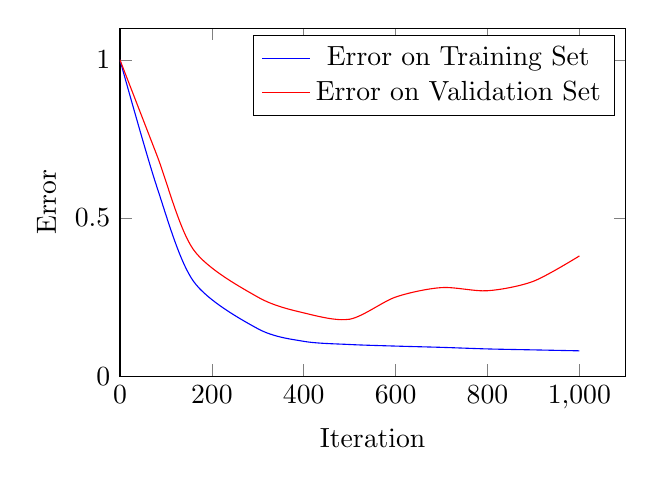
\begin{tikzpicture}
		\begin{axis}[height=6cm,width=8cm,ylabel=Error,xlabel=Iteration,xmin=0,ymin=0]
			\addplot[blue,smooth] coordinates{(0,1)(80,0.6)(160,0.3)(300,0.15)(400,0.11)(500,0.1)(600,0.095)(700,0.091)(800,0.086)(900,0.083)(1000,0.08)};
			\addlegendentry{Error on Training Set}
			\addplot[red,smooth] coordinates{(0,1)(80,0.7)(160,0.4)(300,0.25)(400,0.2)(500,0.18)(600,0.25)(700,0.28)(800,0.27)(900,0.3)(1000,0.38)};
			\addlegendentry{Error on Validation Set}
		\end{axis}
	\end{tikzpicture}
    	\caption[Early stopping based on a validation set.]{The error on the validation set (red) is usually getting larger when the network begins to overfit the training set. Thus, although the error on the training set (blue) is decreasing monotonically, we may want to stop training early to avoid overfitting.}
    	\label{fig:early-stopping}
\end{SCfigure}

\end{document}